\chapter{Treplica Reconfigurável}\label{cap2}

Descrever a proposta e sua implementação.

\section{Visão arquitetural de Treplica}

Introdução da arquitetura de treplica

\subsection{Componentes de suporte}

Comentar sobre a abstração dos componentes de suporte

\subsubsection{Transport}

\subsubsection{Change Log}

\subsubsection{Ledger}

Ledger é a abstração do estado persistente para implementação de Paxos. É uma estrutura
de dados comum, compartilhada por todos os agentes de Paxos, implementados por Treplica,
que conseguem através de uma interface acessar a memória principal. A implementação dessa
interface suporta persistência dos dados de forma não-volátil. Conforme definido no
\autoref{cap1:replicacao_ativa_paxos}, é possível obter o mesmo estado replicado a partir
das instâncias de consenso armazenadas em memória persistente. Assim, a abstração do
Ledger concentra todos os dados de uma instância de consenso bem sucedido em memória
persistente, facilmente acessível a partir da memória principal. A classe LoggingLedger é
o objeto utilizado para persistir em log (disco) as alterações. Para simplificar o uso de
log de alterações, esta implementação tem suporte para detectar e isolar as alterações
feitas em seu estado interno. Pode gravar mudanças no estado e depois recuperá-la,
reaplicando um conjunto de alterações previamente gravados. O Ledger armazena o estado
completo de cada instância do consenso por réplica, mantendo todos os dados exigidos por
todos os tipos de agentes de Paxos implementados por Treplica. Dessa forma, é possível que
qualquer agente recupere seu estado, inclusive o coordenador.

\subsubsection{Secretary}

Secretary apresenta uma abstração unificada de I/O para os agentes de Paxos. Este
componente utiliza memória persistente usando \emph{change log} e o Ledger, lida com a
passagem de mensagens usando o componente de transporte e lida também com a fila de
objetos utilizada para entregar objetos para a aplicação. A principal razão para criação
dessa abstração em Treplica foi sintetizar as operações de I/O em \emph{threads}
diferentes das que executam as operações de Paxos. Operações de I/O em disco, tem grande
potencial para reduzir o desempenho do algoritmo Paxos por duas razões: (1) todas as
requisições de escrita que estabeleceram consenso, devem ser persistidas de forma
não-volátil antes do progresso do algoritmo. Premissa para garantir consistência; (2)
alguns passos do algoritmo de Paxos podem demandar muito acesso a memória persistente.
Considerando que cada operação de escrita em disco leva cerca de $1ms$ para ser concluída
e que uma rodada de Paxos, pelo menos, requer duas escritas em memória estável, acabamos
de adicionar uma latência de $2ms$ em todas as rodadas de consenso.

Uma vez que o I/O é tratado apenas pelo Secretary de forma assíncrona é possível resolver
o problema de falta de paralelismo entre as rodadas. Isso é feito através de uma fila de
agrupamento de gravações lógicas distintas que retém os dados realizar uma única gravação
física. Essa abordagem é vantajosa porque o tamanho dos dados de escrita no disco, utiliza
uma \emph{sync() system call} causando um pouco latência na operação. A implementação d
de Scretary absorve latência da \emph{system call} mantendo uma \emph{thread} separada
para persistência dos dados.

\subsubsection{Router}

Router é um componente simples, mas vital para PaxosPersistentQueue, porque inicia todos
os agentes em conjunto. Sua função principal é prover o \emph{main loop} da implementação
de Paxos, que recebe mensagens do componente de transporte e, de acordo com seu tipo,
encaminha para o agente apropriado. Dessa forma, a execução desse agente é sequencial e
compartilha estruturas de dados, como o Ledger, não precisa de controle de concorrência.

Esse é o único componente (\emph{thread}) que monitora o temporizador central e gera
eventos de \emph{timer} \footnote{Os eventos de \emph{timer} simbolizam a passagem do
tempo para a aplicação. Esse evento atinge todos os componentes que necessitam de um
relógio para seu correto funcionamento}. O código de processamento dos agentes não possuem
operações que geram grandes bloqueios, eles são programados como simples manipuladores de
eventos caracterizando uma arquitetura de processamento assíncrono baseada em eventos
(\emph{event-based}). É responsabilidade do Router instanciar agentes e componentes de
apoio e, também, inicializar a PaxosPersistentQueue.


\subsection{Componentes de Paxos}

Falar sobre a abstração dos componentes de Paxos

\subsubsection{Election}

\subsubsection{Learner}

\subsubsection{Coordinator}

Coordenador (\emph{coordinator}) é o agente responsável por conduzir a rodada de consenso.
Ele é capaz de decidir, através da aplicação de uma regra local, se uma rodada foi bem
sucedida ou não. A regra local do coordenador é baseada em quóruns de \emph{receptores} e
exige que pelo menos $\lfloor n/2 \rfloor + 1$ receptores façam parte de uma rodada, onde
$n$ é o número total de receptores na aplicação \cite{lamport98}.

É permitido a existência de apenas um coordenador por rodada, em caso de falha na réplica
que executa o agente coordenador, uma eleição de líder deve ser convocada para estabelecer
que uma réplica correta execute o agente coordenador. Como o algoritmo é executado no
modelo computacional falha-e-recuperação, a réplica defeituosa pode voltar a computação
acreditando que ainda é o coordenador. Nesse caso, uma nova eleição de líder deve ser
convocada novamente para restabelecer a unicidade de coordenador por rodada.

\subsubsection{Proposer}

Proponente (\emph{proposer}) são agentes capazes de propor valores. Os proponentes podem
propor dois valores diferentes concorrentemente (condição de concorrência)
\footnote{Também conhecida como condição de corrida, acontece quando diferentes processos
em execução atuam sobre um estado compartilhado \cite{alguem}}, nesse caso suas propostas
podem colidir inviabilizando o sucesso de uma rodada de consenso. Em caso de colisões,
diferentes mecanismos podem ser implementados, para lida com essa situação Treplica inicia
uma nova rodada por intermédio do agente \emph{coordenador}.

\subsubsection{Acceptor}


\section{Alterações}

Descrever o objetivo dessa secao

\subsection{Paxos com Réplicas Leitoras}

A ideia principal da abordagem proposta é utilizar réplicas que não participem do processo
de decisão de instâncias de consenso. Isso é feito com a adoção de \emph{réplicas
leitoras}, que são réplicas onde apenas parte dos agentes do algoritmo Paxos estão
executando. Para maior clareza de exposição, quando necessário, chamaremos as réplicas
contendo todos os agentes ativos de \emph{réplicas votantes}. Para suportar a adaptação
elástica a novos perfis de desempenho, desenvolvemos um mecanismo para o
\emph{provisionamento de réplicas} e uma \emph{política de reconfiguração}.

\subsubsection{Réplicas Leitoras}

Réplicas leitoras são réplicas onde apenas os agentes proponente e aprendiz estão
executando. Dessa forma, do ponto de vista do conjunto de processos que implementam o
algoritmo Paxos, uma réplica leitora é capaz apenas de propor operações a serem aplicadas
no estado replicado e de aprender operações decididas pelo conjunto de receptores. Do
ponto de vista do cliente da aplicação replicada um réplica leitora se comporta como uma
réplica votante: ela atende requisições de qualquer tipo garantindo a execução atômica das
mesmas.

As réplicas leitoras não assumem um papel fundamental na execução do algoritmo Paxos, no
entanto elas se integram de forma consistente com a operação das réplicas votantes por
meio de suas funções fundamentais: propor e aprender requisições de escrita. As réplicas
leitoras propõem novas requisições a serem executadas em nome de seus clientes através de
seu agente proponente. O proponente encaminha a operação ao coordenador que por sua vez
decide, em conjunto com os receptores, a ordem da mesma através de uma rodada de Paxos,
como descrito no \autoref{cap1:replicacao_ativa_paxos}. Uma vez que a decisão é alcançada,
a mesma é difundida para o resto do sistema. Nesse momento o agente aprendiz da réplica
leitora toma conhecimento da decisão e atualiza o seu estado interno, sem a participação
ativa do coordenador ou de qualquer receptor.

Tanto o processo de proposta quanto o de aprendizado executado por uma réplica leitora
devem usar as mesmas estratégias de implementação das réplicas votantes. Na verdade, em
nossa implementação usando Treplica, as réplicas leitoras foram construídas a partir da
separação modular dos agentes que implementam Paxos. Dessa forma, reutilizamos os mesmos
componentes e por consequência essas réplicas são capazes de detectar e reenviar propostas
perdidas, detectar e corrigir lacunas na sequência de instâncias de consenso, fazer
controle de fluxo e de congestionamento, entre outras operações fundamentais para uma
operação eficiente de Paxos \cite{vieira-tr10b}.

Uma consequência importante do uso de réplicas leitoras é que essas réplicas,
consistentemente com as funções que elas assumem no algoritmo Paxos, não precisam de
memória persistente para sua operação. Isso se deve ao fato de que elas não executam as
Fases 1 e 2 do algoritmo. Porém, pode ser interessante que essas réplicas registrem a
proposta decidida de forma a não precisar realizar uma recuperação completa em caso de
falha. Na nossa proposta de réplicas leitoras decidimos não fazer esse registro de forma a
remover completamente a escrita em memória persistente do caminho crítico de execução. É
interessante observar que a escrita eliminada ocorre somente quando a réplica leitora
atualiza o seu estado de acordo com as propostas decididas pelos receptores das réplicas
votantes. Dessa forma, as réplicas leitoras conseguem manter seu estado atualizado com as
réplicas votantes com um custo mínimo. Elas também são capazes de processar requisições de
escrita com um custo similar àquele gerado pelas réplicas votantes ao executar as mesmas
requisições. Podemos argumentar que esse custo é menor, na medida que as réplicas leitoras
aliviam as réplicas votantes do custo de manter as conexões abertas com os clientes. É
concebível ainda uma configuração onde as réplicas votantes não entrem em contato com os
clientes, sendo essa operação completamente delegada às replicas leitoras, conforme
ilustra a \autoref{fig:replicas_votantes_protegidas}.

\begin{figure}[ht]
  \begin{center}
    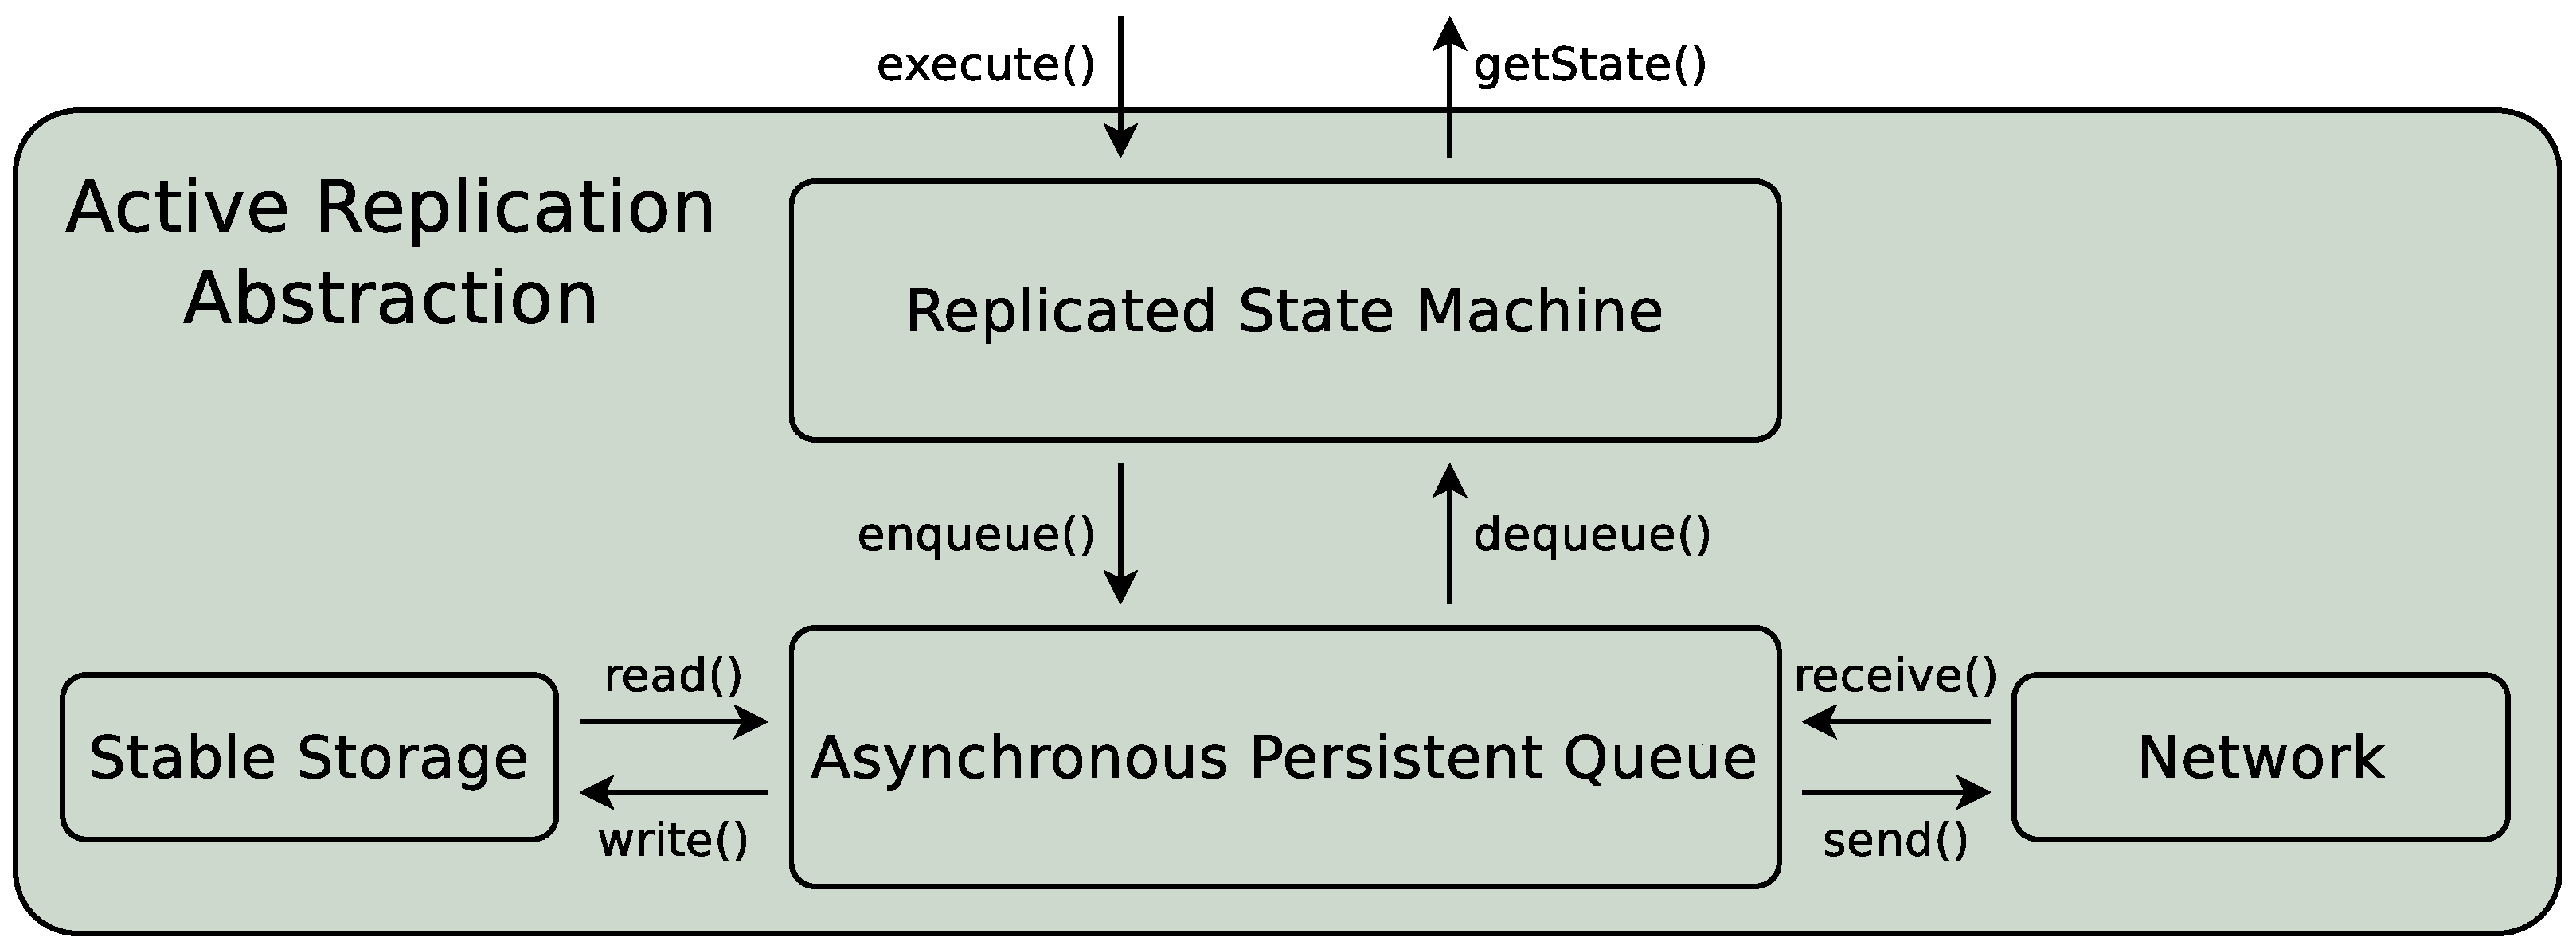
\includegraphics[width=14cm]{conteudo/capitulos/figuras/treplica.eps}
  \end{center}
  \caption{Núcleo de réplicas votantes}
  \label{fig:nucleo_replicas_votantes}
\end{figure}

As réplicas leitoras funcionam então como uma espécie de cache \emph{write-through}
distribuído. O estado replicado na memória destas réplicas permite atender diretamente as
requisições de leitura dos clientes, enquanto as requisições de escrita são repassadas ao
receptores. Podemos ver claramente que a taxa de acerto desse cache está diretamente
ligada à proporção de operações de leitura geradas pelos clientes e que a vazão de
operações de leitura tem o potencial de crescer linearmente com o número de réplicas
leitoras disponíveis. A \autoref{fig:relacao_leitura_escrita} mostra a relação entre as
operações de leitura e escrita.

\begin{figure}[ht]
  \begin{center}
    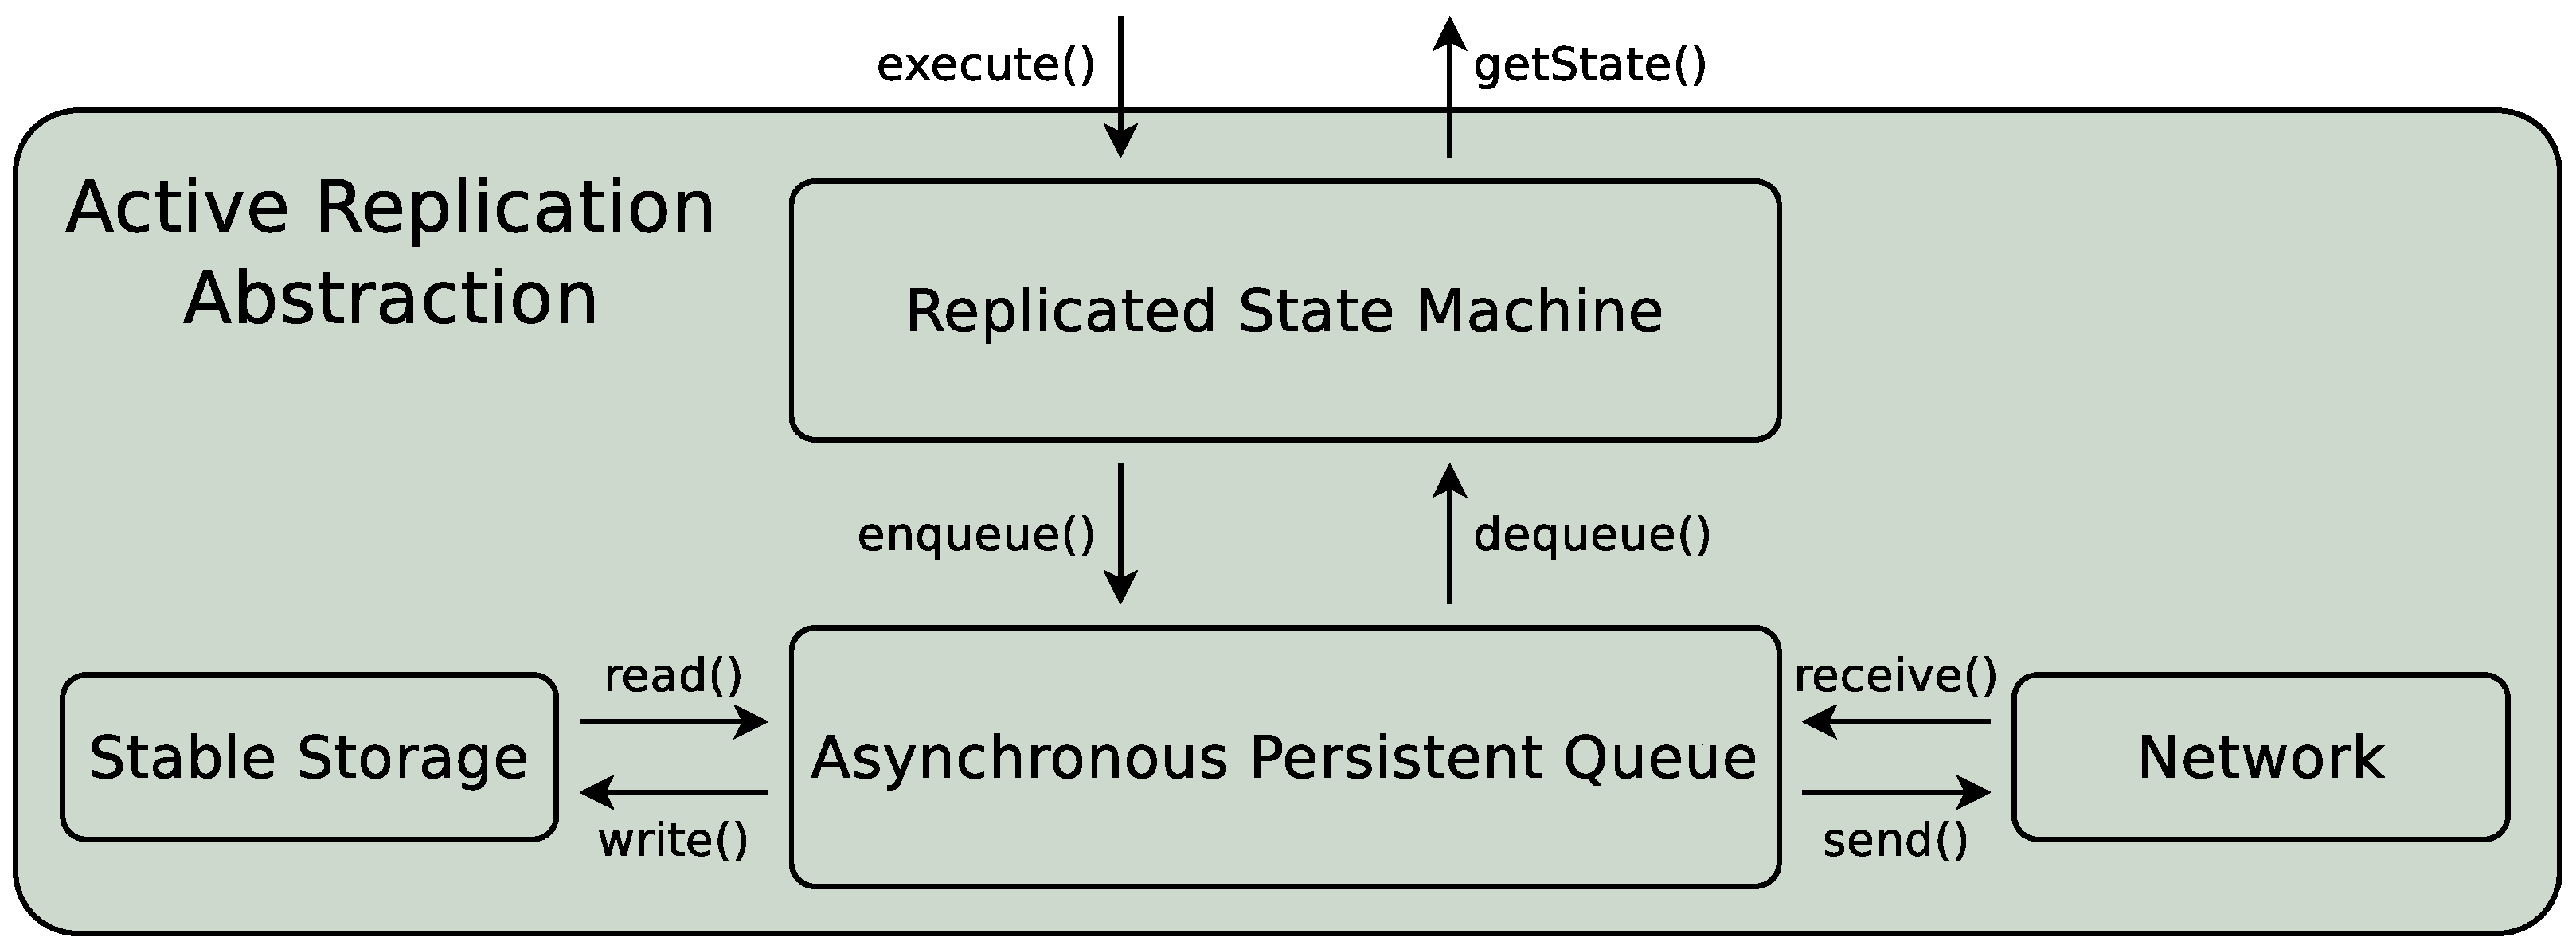
\includegraphics[width=14cm]{conteudo/capitulos/figuras/treplica.eps}
  \end{center}
  \caption{Taxa de acerto do cache}
  \label{fig:relacao_leitura_escrita}
\end{figure}

\subsubsection{Provisionamento de Réplicas Leitoras}

É possível utilizar os mecanismos tradicionais de Treplica para provisionar uma nova
réplica leitora. Em resumo, uma réplica que se integra ao sistema pela primeira vez ou
após uma falha demorada deve recuperar o seu estado. Esse processo acontece através de um
mecanismo de preenchimento de lacunas, que observa que não pode executar novas requisições
de escrita sem antes executar as requisições anteriores \cite{vieira-tr10b}. Esse
procedimento é voltado para reparar pequenas interrupções e não a recuperação do estado
completo de uma réplica. Em particular, no caso de uma réplica leitora sem estado
persistente, o tamanho dessa recuperação pode ser muito grande em termos do número de
\emph{requisições} a serem reexecutadas, pois ela sempre parte do estado inicial vazio.

Foi necessário então criar um procedimento de provisionamento de réplicas, de forma a
permitir o rápido início de uma réplica leitora. Esse mecanismo não é necessariamente
exclusivo de réplicas leitoras e pode ser aplicado a réplicas normais. Porém, neste
primeiro momento, ele tira proveito do fato dessas réplicas não terem memória persistente.
Em particular, a adição ou remoção de uma réplica leitora não altera o número de
receptores executando o algoritmo, não havendo necessidade de se realizar um
reconfiguração custosa \cite{lamport10}.

\subsection{Protocolo para transferência de estado}
...


\subsection{Alterações Propostas - Componente n}

:se...
